Beyond all the planning of the concerns of the project, it is profitable to outline a initial planning for the accomplishment of the project. It can be beneficial because, in a certain way, forces the definition of some tasks and also allows the correct division of the time given the difficulties of these tasks. That being said, a more methodical and organized approach can be followed.


\begin{figure}[!hb]
\centerline{
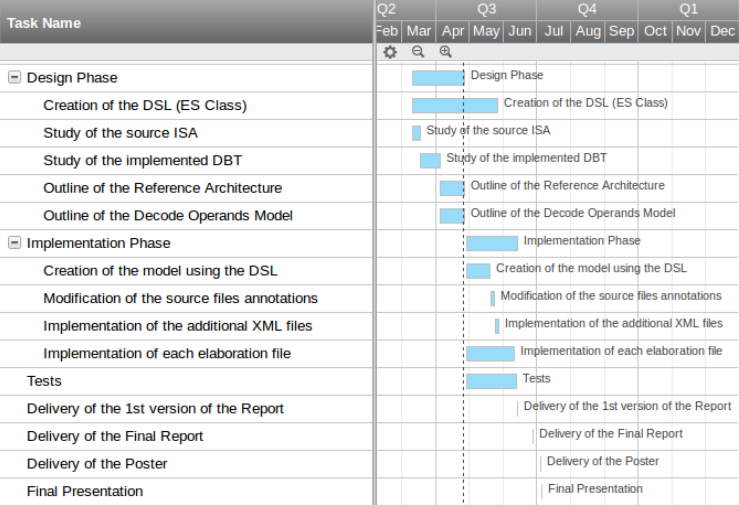
\includegraphics[scale=0.6]{images/planning}}
\caption{Gantt Diagram for the project (post Analysis)}
\label{fig:planning} 
\end{figure}

So, according to our planning, the tasks that can take some of the time are the development of the modelization language, since that it is a project that is being developed from scratch by the entire Embedded Systems class, the study and definition of the conceptual model of the \textit{DBT} and the implementation of the elaboration files as well as the implementations of all the behaviors that the decoder can have, which will be explained rigorously later in this report. 








